%% LyX 2.2.3 created this file.  For more info, see http://www.lyx.org/.
%% Do not edit unless you really know what you are doing.
\documentclass[english]{upeeei}
\usepackage[latin9]{inputenc}
\setcounter{secnumdepth}{3}
\setcounter{tocdepth}{3}
\synctex=-1
\usepackage{babel}
\usepackage{array}
\usepackage{url}
\usepackage{multirow}
\usepackage{graphicx}
\usepackage[unicode=true,pdfusetitle,
 bookmarks=true,bookmarksnumbered=false,bookmarksopen=false,
 breaklinks=false,pdfborder={0 0 1},backref=false,colorlinks=false]
 {hyperref}

\makeatletter

%%%%%%%%%%%%%%%%%%%%%%%%%%%%%% LyX specific LaTeX commands.
%% Because html converters don't know tabularnewline
\providecommand{\tabularnewline}{\\}

%%%%%%%%%%%%%%%%%%%%%%%%%%%%%% Textclass specific LaTeX commands.
\providecommand*{\code}[1]{\texttt{#1}}

%%%%%%%%%%%%%%%%%%%%%%%%%%%%%% User specified LaTeX commands.
\usepackage{colortbl}
%\usepackage{underscore}
%\usepackage{graphicx}
\errorcontextlines 10000

\makeatother

\usepackage{listings}
\begin{document}
%% UP EEEI undergraduate project proposal template
%% adapted from the
%% UP EEEI undergraduate project template
%% v0.1 by Louis P. Alarcon 11/22/2011
%%
%% LyX template - use with the following files:
%% 	uct10_new.clo, uct11_new.clo, uct12_new.clo, upeeei.cls, upeeei.layout
%%
%% Place project title here
\title{Improving Data Center Network Performance through Path Diversity} 

%%
%% Author information

\author{
Charles Joshua Alba\\ 2013-06878\\ \emph{B.S. Computer Engineering} \\\\\\
Kyle Dominic Gomez\\ 2013-25650\\ \emph{B.S. Computer Engineering} \\\\\\
Rene Josiah Quinto\\ 2013-14854\\ \emph{B.S. Computer Engineering}
}

%%
%% Month and year of submission/graduation
\degreeyear{2018} 
\degreesemester{March} 

% Put your advisers here:
\chair{Professor Roel Ocampo}
\othermembers{Professor Isabel Montes} 
\numberofmembers{1} 

\field{Computer Engineering} 
\campus{Diliman} 

\maketitle 

\begin{abstract} 

%Your abstract goes here...
Datacenter networks allow the operation of Internet services by partitioning requests to multiple servers, and aggregating results back to form the response sent to the users. This requires servers within the datacenter to communicate efficiently and rapidly. Services, differentiated by their workload profiles, require a network that can guarantee high throughput, and low flow completion time. To achieve these, this paper focuses on Multipath TCP (MPTCP) as a transport protocol in the context of datacenters, by making better use of the network topology. In addition, changes in the packet forwarding protocol within network switches and the Generic Offload Receiver (GRO) layer within network servers will be employed to make up for MPTCP's undesired behavior within datacenters such as network link hotspots. 
With this, we hypothesize an increase in throughput and decrease in the flow completion time. To test this, we created a simulated datacenter environment wherein various tests were done to measure throughput, goodput, flow completion time, and mean network utilization. Different parameters were changed during the tests to gather data on their respective performance. These parameters are payload size, network traffic conditions, switch forwarding protocol, and reorder resiliency in hosts.
Analyzing the data, the study found that packet spraying turned out to be beneficial for the network in terms of throughput, goodput, and mean network utilization. Reorder resiliency, on the other hand, resulted in a decrease in the performance of the network.

\abstractsignature\end{abstract}

\begin{frontmatter} 

\setlength{\parskip}{0pt}

\tableofcontents{}

\listoffigures

\listoftables

\end{frontmatter} 

\def\MASTERDOC{true}

\cleardoublepage{}

\chapter{Introduction\label{cha:Introduction}}

To keep up with increasing demand for online services, requests and
operations are usually serviced by partitioning tasks into multiple
servers within a datacenter. These servers are then arranged in a
special topology to ensure quick intercommunication between each other,
regardless of packet stream length or size. As a consequence, servers
have multiple paths between each other. There lies a promising performance
benefit by taking advantage of this path diversity, in which the traditional
transport protocol, TCP, cannot provide. 

\section{Servicing Increasing Demand with Datacenter Networks}

Several companies and institutions (Google, Amazon, and Microsoft,
to name a few) provide a wide variety of online services such as video
streaming, online gaming, VoIP, file sharing, and simple web searching.
These online services usually differ in their workload profiles \cite{geng2016juggler,he2008toward}\textemdash faster
connections result to better performance for file sharing services,
while connection stability is the main concern for video streaming
services.

The demand for online services has been increasing steadily due to
their popularity. Moreover, the competitive market have pushed for
innovations to improve services, resulting in increased computational
load \cite{barroso2013datacenter}. To keep up with demand that increases
in both quantity and complexity, companies need to expand and upgrade
their resources, increasing costs \cite{wilson2011better,decandia2007dynamo}.
One way to meet this demand is to distribute service requests to multiple
servers, then aggregating responses to form the final result (also
known as the partition/aggregate design pattern) \cite{alizadeh2010data}.
Infrastructures built with this demand distribution property are called
datacenter networks (DCNs). 

Apart from meeting the increasing demand, this provides several benefits.
Firstly, by having redundant servers, services can be maintained even
during partial network maintenance \cite{barroso2013datacenter}.
Secondly, an organized and redundant network infrastructure eases
management \cite{barroso2013datacenter}. Finally, distributing requests
to different servers increases server utilization, proving to be more
cost-effective and scalable \cite{greenberg2008cost}. 

\section{Connection-Rich Nature of Datacenter Network Topologies }

Partitioned requests are distributed among servers within a datacenter
(end-hosts) through packet streams (flows). Since majority of the
flows stay within a datacenter \cite{benson2010network}, the network
topology must guarantee a speedy and reliable connection between local
end-hosts. These properties can be characterized with sufficient interconnection
bandwidth \cite{al2010hedera,al2008scalable} and fault-tolerance
\cite{niranjan2009portland}. 

Requests must be serviced quickly and aggregated back to the user,
which means that the server response delays also add up and affect
the performance of the service \cite{alizadeh2010data}. End-hosts
also need to keep their internal data structures fresh \cite{alizadeh2010data}
through frequent large transfers of data. Therefore, datacenters must
also guarantee low latency for short flows, and high throughput to
service large flows \cite{alizadeh2010data,he2008toward}. 

Current datacenter network topologies guarantee the previous characteristics
through different approaches. Switch-centric topologies \cite{al2008scalable,leiserson1985fat}
rely solely on switches and routers to forward traffic across the
network, which ensures speedy delivery due to specialized hardware
at the expense of scalability. Server-centric topologies \cite{guo2008dcell,guo2009bcube}
allow servers to forward packets as well, however software routing
may be slow and can affect host-based applications \cite{lebiednik2016survey}.

Topologies can be also designed to be modular \cite{guo2009bcube}
or hierarchical \cite{leiserson1985fat} to increase network capacity
through scalability \cite{al2010hedera}. This introduces multiple
redundant links and paths between servers within the network, establishing
a connection-rich nature \cite{he2008toward,rost2003rate}.

\section{Better Network Utilization through Multiple Paths}

Host-to-host connectivity within a datacenter was originally facilitated
using the Transmission Control Protocol (TCP) \cite{alizadeh2010data,raiciu2011improving}.
TCP ensures robustness in the delivery of packets between end-hosts
in the presence of communication unreliability \cite{postel1981transmission}. 

TCP connections make use of a single network path between end-hosts
\cite{kurose2005computer}. Since it is typical for two end-hosts
in a datacenter network to have multiple paths, TCP is unable to fully
utilize the available paths between end hosts \cite{ford2011architectural},
and may not be able to achieve optimal network utilization. 

To make use of the available resources in a path-diverse network,
Multipath TCP (MPTCP) was proposed as an experimental protocol by
the IETF. MPTCP uses parallel TCP connections \cite{ford2013tcp,fordmptcpslides},
which increases throughput and resiliency of the network \cite{ford2011architectural}.

\section{Outline of the Document}

The rest of the document is presented as follows. The next chapter
will discuss different improvements suggested for MPTCP based on different
metrics such as reliability, and a global view of the network. Additionally,
some issues in unmodified MPTCP are also discussed and studied in
depth. Chapter 3 discusses the problem statement, objectives, and
scope and limitations of the project. Section 4 and 5 discuss the
steps taken to create the project. 

\cleardoublepage{}

\chapter{Review of Related Work\label{cha:RRW}}

While MPTCP promises performance benefits such as increased throughput
between two hosts, it suffers from problems which hinder or negate
its advantages. The nature of datacenter network traffic and topology
presents two potential setbacks for MPTCP. First, short packet streams
(short flows) might experience a higher latency due to MPTCP's connection
establishment mechanism. Second, large packet streams (large flows)
might suffer from lower throughput due to MPTCP's congestion and subflow
mechanism. In addition to the presented solutions to these problems,
a closer look is given to switch-based packet spraying, combined with
host-based reordering resiliency, as a potential improvement over
MPTCP. 

\section{Connection Establishment of MPTCP Penalizes Short Flows }

MPTCP, being designed as an extension for TCP \cite{ford2013tcp},
inherits its congestion control mechanisms. One of which is Slow Start
\cite{stevens1997tcp}, where each subflow starts sending a limited
amount of packets, then exponentially increases its sending rate until
a link capacity/threshold is reached. Exceeding link capacity can
result to packet loss due to switch overflows, making the receiver
fail to acknowledge the packet. This subsequent action will cause
the sender to retransmit the packet due to its internal retransmission
timeout, or due to receiving three duplicate acknowledgements (TCP
Fast Retransmit) for a previously sent packet, in addition to reducing
the sending rate of the sender. 

Since majority of the flows on a datacenter are short flows \cite{greenberg2009vl2}
and are of a bursty nature \cite{alizadeh2010data}, MPTCP would cause
these flows to stay in the Slow Start phase \cite{barik2016lisa},
where the sending rate is initially limited, then is increased drastically.
Therefore, when short flows lose packets due to congestion, retransmission
is necessary, and this increases the flow completion time \cite{kheirkhah2016mmptcp}.

In addition, MPTCP also inherits TCP's handshake protocol, in order
to create and establish subflows between end-hosts. Since MPTCP cannot
discern between short and long flows, it cannot decide as to how many
subflows should be established to optimally send packets across the
network. Therefore, a mismatch in the number of subflows, specifically
for short flows would further increase the flow completion time due
to the extra packets required to establish a connection.

To minimize the flow completion time for short flows, connections
can start by spraying packets over multiple paths. Connections then
can switch back to MPTCP upon reaching a certain amount of packets
\cite{kheirkhah2016mmptcp}, to make use of MPTCP's benefits over
long flows such as increased throughput and better congestion control.
However, the introduction of packet spraying in addition to using
MPTCP would open this specific implementation to both problems associated
with each. 

\section{Decreased Throughput due to Redundant Retransmissions }

MPTCP uses Equal-Cost Multipath (ECMP), a switch-based algorithm,
to forward packets through the network \cite{raiciu2011improving}.
ECMP bases its forwarding on a 5-tuple (source IP, destination IP,
source port, destination port, protocol number) \cite{hopps2000multipath}
which is hashed and used to forward packets to paths. This means that
all data belonging to one subflow will strictly follow one network
path. Selected network paths by ECMP may traverse links that have
already been chosen by another subflow, which will effectively decrease
the maximum available capacity of the link. Areas in the network that
are close to exceeding link capacity are called hotspots. Colliding
subflows may exceed the link capacity for any given link in a datacenter
network, resulting in full switch queues. Full switch queues will
then lead to dropped packets, which in turn, decrease mean network
utilization \cite{al2010hedera}.

Duplicating packets across multiple paths (bicasting/multicasting)
in an MPTCP connection can be used to mitigate the decrease in throughput
due to dropped packets \cite{fukuyama2016throughput}. In full bicasting,
each connection transmits a copy of all packets sent across multiple
subflows, while selective bicasting only duplicates packets that are
sent as a retransmission of lost packets. 

However, the increase in throughput for individual subflows brought
about in both full and selective bicasting may not be optimal in a
datacenter. This is, in part, attributed to the duplicating nature
of bicasting wherein redundant data is sent through the network's
links and consumes resources for other subflows. In addition to redundant
data packets, control packets such as the ACK packets in TCP add to
network traffic. This added traffic to the network can be perceived
as a loss in throughput. 

\section{Diffusing Network Hotspots through MPTCP with Packet Spraying }

As previously mentioned, network hotspots create areas of congestion
in datacenter networks, throttling the throughput of the connections
that pass through these hotspots. One way to avoid this is to use
packet spraying \cite{dixit2013impact}. Packet spraying spreads a
sequence of packets through different candidate ports instead of forwarding
packets of a single flow through a chosen port according to its hashed
flow identifier as seen in ECMP. This scheme prevents the collision
of multiple paths onto specific links (hash collision), and spreads
the packets in the hopes of evenly distributing the load through all
relevant links of the network. 

However, distributing packets of a flow into different paths can lead
to out-of-order packets if the paths have significantly different
end-to-end delays \cite{dixit2013impact}. End-hosts receiving packets
that do not arrive in the order that they were sent may falsely perceive
that the network is lossy and request for retransmissions \cite{postel1981transmission}.
The sending end-host will receive these retransmission requests and
will falsely perceive that there is congestion in the network, cutting
the congestion window in half which will then result in the reduction
of throughput.

One way to avoid false congestion due to packet reordering is to adjust
the time threshold of the end-hosts before they request for retransmission
\cite{kheirkhah2016mmptcp}, effectively making end-hosts more tolerant
to delays in the network. However, an improper configuration (mismatch)
of this threshold will result in an increased delay before sending
retransmission requests in actual congestion experienced in the network,
greatly decreasing the flow completion time and penalizing short flows.

To increase the resiliency of the end-hosts against out-of-order packets
while avoiding a threshold mismatch, one solution would be to increase
the buffer size of the Generic Receive Offload (GRO) layer of the
end-hosts \cite{zhang2017resilient}. The GRO layer works underneath
the transport layer, and is responsible for bundling packets to decrease
computational overhead versus individual per-packet processing. Increasing
the buffer size enables it to accept packets that arrive earlier than
those preceding it thereby increasing its resilience towards out-of-order
packets. This is based on the assumption that, in a datacenter, delay
differences between paths are significantly less than in non-datacenter
networks.

\section{Drawbacks Caused by MPTCP with a Global View }

With Software Defined Networking (SDN), a global view of the network
state can be provided to a central controller \cite{nunes2014survey,kim2013improving,yeganeh2013scalability}.
This enables network protocols to make use of global network information,
such as link utilization and end-to-end delays \cite{hussein2017sdn,zannettou2016exploiting},
to create more informed decisions. SDN approaches have introduced
several benefits to MPTCP, such as increased throughput and network
resiliency, by controlling the number of subflows and scheduling the
routes of different connections to avoid both network hotspots and
out-of-order packets \cite{hussein2017sdn}. 

These benefits, however, comes at the price of controller overhead
\cite{hussein2017sdn}. SDN controllers need to communicate regularly
with the network switches in order to issue forwarding rules to adapt
with the situation, causing delays. Since most congestion events that
happen in datacenter networks are because of traffic bursts that only
lasts for a few microseconds (microbursts) \cite{ghorbani2017drill},
controller overhead becomes significant, and so SDN implementations
cannot respond fast enough. Due to controller overhead, SDN implementations
can also increase the flow completion time of connections, penalizing
short flows. Moreover, SDN implementations generally do not scale
with a large number of connections as the controller overhead also
increases with the number of active connections \cite{hussein2017sdn}.

\cleardoublepage{}

\chapter{Problem Statement and Objectives \label{cha:ProbStatement}}

\section{Problem Statement}

Common topologies in datacenter networks exhibit symmetry and path
diversity \cite{he2008toward}. This ensures that multiple paths of
equal costs exist between two end-hosts \cite{dixit2013impact}. In
addition, an ideal datacenter network must guarantee high throughput
for large flows, and low latency for short flows \cite{alizadeh2010data,he2008toward}.

Multipath TCP (MPTCP), an experimental protocol by the IETF, is a
TCP extension that uses multiple paths over many connections \cite{ford2013tcp}.
By using multiple paths simultaneously, MPTCP aims to increase network
utilization, specifically throughput, and increase \char`\"{}resilience
of connectivity\char`\"{} \cite{fordmptcpslides}. This is done by
employing Equal Cost Multi-Path (ECMP) \cite{raiciu2011improving},
a switch-based forwarding algorithm. ECMP hashes subflows into separate
paths using the packet's header information. However, hotspots in
the network may occur when flows are hashed to paths with one or more
links overlapping with each other \cite{al2010hedera}, usually exceeding
the link capacity. Because of this, the network experiences a drop
in network utilization due to sender backoff \cite{dixit2013impact}. 

Random packet spraying, an alternative to ECMP, can be used to resolve
hotspots as it allows for a greater granularity for load balancing
\cite{he2008toward}. However, this can result in reordered packets
at the receiver, triggering false retransmissions upon receipt of
three duplicated packet acknowledgements \cite{ford2011architectural},
in addition to drastically reducing sender throughput \cite{zhang2003rr}.
This can be minimized by dynamically changing the retransmission threshold.
However, a positive mismatch on the threshold may mean a slower response
time for actual packet drops \cite{zhang2003rr}.

Minimizing retransmission due to out-of-order packets can be done
by supplementing the function of the Generic Receive Offload (GRO)
layer to fix the order of packets \cite{geng2016juggler} in addition
to merging packets together. This not only reduces computational overhead
compared to per-packet processing, but makes the end-hosts more tolerant
to packet reordering, and thus reduces retransmissions. However, reordered
packets must arrive within a short delay of each other since the switch
queues are limited and timeouts are smaller. 

Also, to maintain backwards compatibility with TCP, MPTCP also suffers
from the complexity in connection establishment \cite{dixit2013impact}
and slow start \cite{stevens1997tcp}, which in turn penalizes short
flows through higher flow completion times. To maintain lower flow
completion times and lower latency for short flows, a specified amount
of packets are sprayed through multiple paths initially before switching
to MPTCP \cite{kheirkhah2016mmptcp}. However, this means that it
inherits problems from both implementations altogether. 

Better network utilization can be also achieved using Software-Defined
Networking \cite{hussein2017sdn,zannettou2016exploiting} with MPTCP.
With a global view of the network, it can better utilize path diversity,
have a better gauge on the number of subflows per connection, and
ideally minimize the receipt of out-of-order packets. This solution
benefits large data flows, but due to the added controller overhead,
it may penalize short flows. In addition, it may also have some scalability
issues \cite{zannettou2016exploiting}.

To combat delay and lower throughput caused by multiple timeouts on
wireless networks, retransmission redundancy was implemented using
full and partial bicasting over MPTCP \cite{fukuyama2016throughput}.
This may not necessarily be effective in the datacenter setup as redundant
packets may cause more false retransmissions. 

We hypothesize that an increase in overall throughput and network
utilization in MPTCP can be achieved through implementing packet spraying
in the network instead of ECMP. Since packet spraying can introduce
an eventual decrease in throughput, we hypothesize that this can be
mitigated by creating reorder-resilient end hosts. By comparing the
results we see from different experiments, we strengthen the basis
for considering a reorder-resilient network for future datacenter
networks, as well as potentially contribute to the growth of MPTCP
as an experimental protocol.

\section{Objectives}

The objectives of this work are as follows: First is to experimentally
prove that MPTCP benefits large flows, but penalizes short flows.
Next, understand and prove that network hotspots occur due to ECMP-based
switches. Lastly, observe and analyze the effects of packet spraying
switches, as well as reorder-resilient hosts, to minimize network
hotspots, and in turn benefit both short and large flows.

\section{Scope and Limitation}

The project will focus on datacenter networks, and assume ideal working
conditions. More specifically, this project does not consider the
possibility of switch failures, host failures, link damages that could
cause degradation of performance or even disconnections. Among datacenter
topologies, only fat tree topologies and possible variants will be
considered. 

While the nature and topology of datacenter networks are highly distinct
from the vast majority of the Internet, or wide area networks (WANs),
the results and observations presented in this paper may potentially
apply to WANs as well.

As this paper relies heavily on experiments done through network simulations,
this project cannot guarantee the realization of actual or realistic
datacenter network traffic, but tests will be made to mimic certain
datacenter network conditions such as worst-case scenarios. 

\cleardoublepage{}

\chapter{Methodology\label{cha:Methodology}}

Taking into consideration the penalties incurred on short flows from
MPTCP connection establishment complexity, as well as the penalties
incurred on long flows due to the network hotspots that arise as a
consequence of ECMP routing, we chose to measure flow completion time,
and end-host throughput and goodput, respectively. Mean network utilization
was also measured to gauge the effectivity of each protocol in terms
of how well the available network routes were used.

To properly attribute each change in the above metrics, several possible
permutations of the routing behavior, transport protocol, flow types
(or payload sizes) end-host pairs, and network conditions were tested.
These metrics were extracted and compared against each other considering
the varying parameters between each test.

\section{Preliminary Work}

Smaller tests using MPTCP were done to further increase the researcher's
understanding of the protocol and its interaction with Mininet. MPTCP
was confirmed to be working as indicated in the laboratory experiment
of an SDN class \cite{ke2016mptcplab}. An overview of the topology
can be found in Figure \ref{fig:Mininet-topology}. To simplify things,
router \code{r2} is configured to forward packets, acting as a router\footnote{From this point onwards, we use the terms switch and router interchangeably
to mean devices that do layer 2 forwarding and layer 3 routing.}. All links are capped at a speed of 10 Mbps (i.e., the minimum supported
transmission rate of both devices connected to the link is 10 Mbps).

\begin{figure}
\begin{centering}
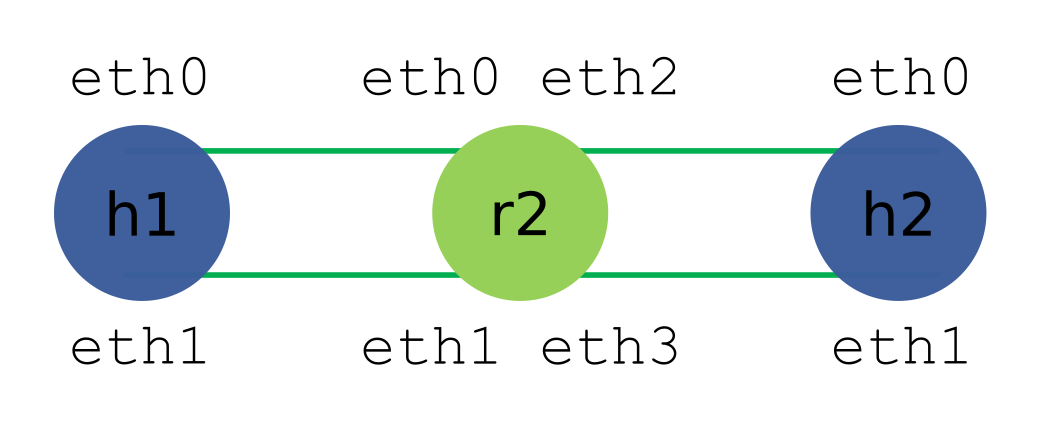
\includegraphics[scale=0.2]{basictopo}
\par\end{centering}
\caption[Mininet topology for MPTCP tests.]{Mininet topology for MPTCP tests. Links are of 10 Mbps speed. Topology
copied from \cite{ke2016mptcplab}\label{fig:Mininet-topology}}
\end{figure}

\subsection{Managing Multipath TCP Subflows}

In the preliminary setup and tests, it was found that MPTCP can be
configured using different parameters. MPTCP handles the discovery,
setup, and termination of subflows through the heuristics of a path
manager \cite{postel1981transmission}. We considered three of the
four available path managers that MPTCP provides \cite{uclouvain2017configure}. 

First, the default path manager does not initiate nor announce different
IP addresses, but will still accept subflows from end-hosts that do.
Next, the full mesh path manager creates flows using all combinations
of interfaces (device within end-host to connect to links \cite{coltun2008rfc})
of both end-hosts (i.e. assuming all interfaces correspond to unique
IP addresses, two end-hosts with three interfaces each will have 9
subflows). Finally, the n-different-ports path manager allows the
control over the number of subflows in a connection through the use
of different ports. The fourth path manager called binder, isn't considered
as it was designed for mobility of devices, a trait not present in
datacenter networks.

In summary, we see the comparisons of MPTCP path managers in Table
\ref{tab:Path-Manager-Comparison}. To serve as a control group, TCP
was characterized as well.

\begin{table}
\noindent\resizebox{\textwidth}{!}{%
\begin{tabular}{|c|c|c|>{\centering}p{4cm}|>{\centering}p{4cm}|>{\centering}p{4cm}|}
\hline 
Routing Protocol & Path Manager & Initiates subflow creation & Number of used IP address pairs & Number of used port number pairs & Number of subflows\tabularnewline
\hline 
\hline 
TCP & None & N/A & 1 & 1 & 1\tabularnewline
\hline 
MPTCP & default & No & As sender: 1 As receiver: based on sender  & As sender: 1 As receiver: based on sender  & As sender: 1 As receiver: based on sender \tabularnewline
\hline 
MPTCP & fullmesh & Yes & All, combination & Configurable, default is 1  & \code{No. of source IP-port pairs {*} No. of destination IP-port pairs}\tabularnewline
\hline 
MPTCP & ndiffports & Yes & 1 & Corresponds to number of subflows  & Configurable, default is 2\tabularnewline
\hline 
\end{tabular}

}\caption{Comparison of MPTCP path managers and TCP.\label{tab:Path-Manager-Comparison}}
\end{table}

\subsection{Validating the Behavior of MPTCP Path Managers}

Considering the topology described in Figure \ref{fig:Mininet-topology},
we expect to see TCP, default MPTCP, and ndiffports MPTCP to have
a sender rate of 10 Mbps, whereas Full Mesh MPTCP can have a sender
rate of up to 20 Mbps. This is because the first three would only
use 1 IP address pair, and thus is limited to 1 subflow. But, the
Full Mesh MPTCP establishes four subflows, because both hosts have
two available interfaces, fully using all possible links. This was
validated experimentally and the results are shown in Table \ref{tab:Comparison-of-sender}. 

\begin{table}
\begin{centering}
\begin{tabular}{|c|c|}
\hline 
Routing Protocol/Path Manager & Sender throughput (in Mbits/sec)\tabularnewline
\hline 
\hline 
TCP & 9.78\tabularnewline
\hline 
Default MPTCP & 9.43\tabularnewline
\hline 
Ndiffports MPTCP & 9.46\tabularnewline
\hline 
Full mesh MPTCP & 19.1\tabularnewline
\hline 
\end{tabular}
\par\end{centering}
\caption[Comparison of sender throughput between MPTCP path managers and TCP.]{Comparison of sender throughput between MPTCP path managers and TCP.
The topology used was described in Figure \ref{fig:Mininet-topology}.
Throughput values were taken using command line tool \textit{iperf}.
\label{tab:Comparison-of-sender}}
\end{table}
However, using more subflows may sometimes come at a cost. For short
flows, opening multiple subflows may not be necessary, as the packets
may have already been sent even before a new subflow has been established.
To prove that MPTCP does indeed introduce some overhead for short
flows, the flow completion time was measured between TCP, Default
MPTCP, and Full mesh MPTCP.

This experiment once again uses the topology in Figure \ref{fig:Mininet-topology}.
The left host (\code{h1}) will request for the web page from the
right host (\code{h2}), which has a web server running. The web page
to be fetched is a default directory index page, and because the web
server sends a stream of small packets to complete the request, it
counts as a short flow. The tests were ran 10 times with TCP, default
MPTCP, and full mesh MPTCP, and the flow completion time (FCT) were
noted. We defined the flow completion time as the time difference
between the first \code{SYN} packet up to the last \code{ACK} packet
for the last \code{FIN} packet.

\begin{table}
\begin{centering}
\noindent\resizebox{\textwidth}{!}{%
\begin{tabular}{|c|c|c|}
\hline 
Routing protocol/Path Manager & FCT (Mean, in ms) & FCT (Standard Deviation, in ms; Relative Standard Deviation)\tabularnewline
\hline 
\hline 
TCP & 7.86 & 1.53 (19.51\%)\tabularnewline
\hline 
default MPTCP & 8.39 & 1.10 (13.11\%)\tabularnewline
\hline 
full mesh MPTCP & 10.5 & 3.86 (36.70\%)\tabularnewline
\hline 
\end{tabular}
\par\end{centering}
\begin{centering}
}
\par\end{centering}
\centering{}\caption{Mean, standard deviation, and relative standard deviation of flow
completion time for different MPTCP path managers and TCP.\label{tab:fct-tests}}
\end{table}

A summary of results are shown on Table \ref{tab:fct-tests}. Here,
we see that TCP has the fastest flow completion time. As default MPTCP
works much like TCP, but has an added establishment overhead over
TCP, it has a slower flow completion time. Lastly, since full mesh
MPTCP opens multiple subflows while transmitting data, packets for
connection establishment of other subflows compete for the same available
links, resulting in the slowest flow completion time. In addition,
since flows are terminated like TCP connections, extra packets are
sent to terminate all open subflows before finishing.

As the topology considered for the previous experiments is relatively
simpler compared to actual datacenter topologies, we hypothesize that
the observed behavior will still hold true, and the effects are amplified
to a certain extent.

\section{Building the Test Environment}

Mininet was chosen to orchestrate the virtual network, its switches,
and its hosts. The network topology is generated programmatically,
and switch behavior can be swapped through configuration files. It
also ensures that all virtual hosts are running on the same configuration
as the server it is running in. This ease of use allows the researchers
to implement multiple changes at once.

MPTCP is available as an ns-3 model \cite{kheirkhah2014ns3} or a
kernel patch \cite{uclouvain2017mptcp}. Juggler \cite{geng2016juggler},
which modifies the GRO function to fix packet ordering, is only readily
available as a kernel patch. Since the experiments require hosts that
require both features to be present, it was decided that the kernel
patches were to be used. The MPTCP and Juggler custom kernels were
merged together and applied to the server to virtualize certain hosts.

Switches, on the other hand, can be described with its normal forwarding
algorithm, which stores only one next-hop for all destinations in
its routing table. However, the switches must also be capable of Equal
Cost Multi-Path (ECMP), and Packet Spraying (PS), which require a
routing table storing multiple next-hops. Since these forwarding behavior
require inspection into packet headers and metadata, we utilized and
modified software switches enabled by P4, a programming language used
to process packets \cite{bosshart2014p4}.

\pagebreak{}

\subsection{Testbed Specifications}

Experiments and tests were ran on two SuperMicro bare metal servers
with the specifications listed below. One server will be patched with
the MPTCP custom kernel only, and the other with the merged MPTCP
and Juggler kernel.

\begin{table}
\begin{centering}
\begin{tabular}{|c|c|}
\hline 
Technical Specifications & Value\tabularnewline
\hline 
\hline 
Processor & Intel(R) Core i7-3612QE\tabularnewline
\hline 
Processor Speed & 2.10 GHz\tabularnewline
\hline 
Number of Cores & 4\tabularnewline
\hline 
RAM & 16 GB\tabularnewline
\hline 
Operating System & \code{Ubuntu 16.04.3 LTS}\tabularnewline
\hline 
Linux Kernel & \code{Linux version 4.9.60.mptcp}\tabularnewline
\hline 
\end{tabular}
\par\end{centering}
\centering{}\caption{Testbed Technical Specifications.\label{tab:testbed-specs}}
\end{table}

\subsection{Setting up the Network Topology}

For this experiment, the fat tree topology was chosen, a common and
scalable data center network topology. Like all DCN topologies, the
fat tree topology provides several equal cost paths between any two
end-hosts. Moreover, because of the symmetry of the topology even
with scaling, a Mininet topology can be easily set up with unique
addressing \cite{al2008scalable}. Mininet was used for the simulation
of the nodes, and Python was used to construct the topology (See Figure
\ref{code-topogen}) A $K=4$ fat tree topology can be seen in \ref{fig:k-4-topology},
complete with the conventions used. 

\begin{figure}
\begin{centering}
\noindent\resizebox{\textwidth}{!}{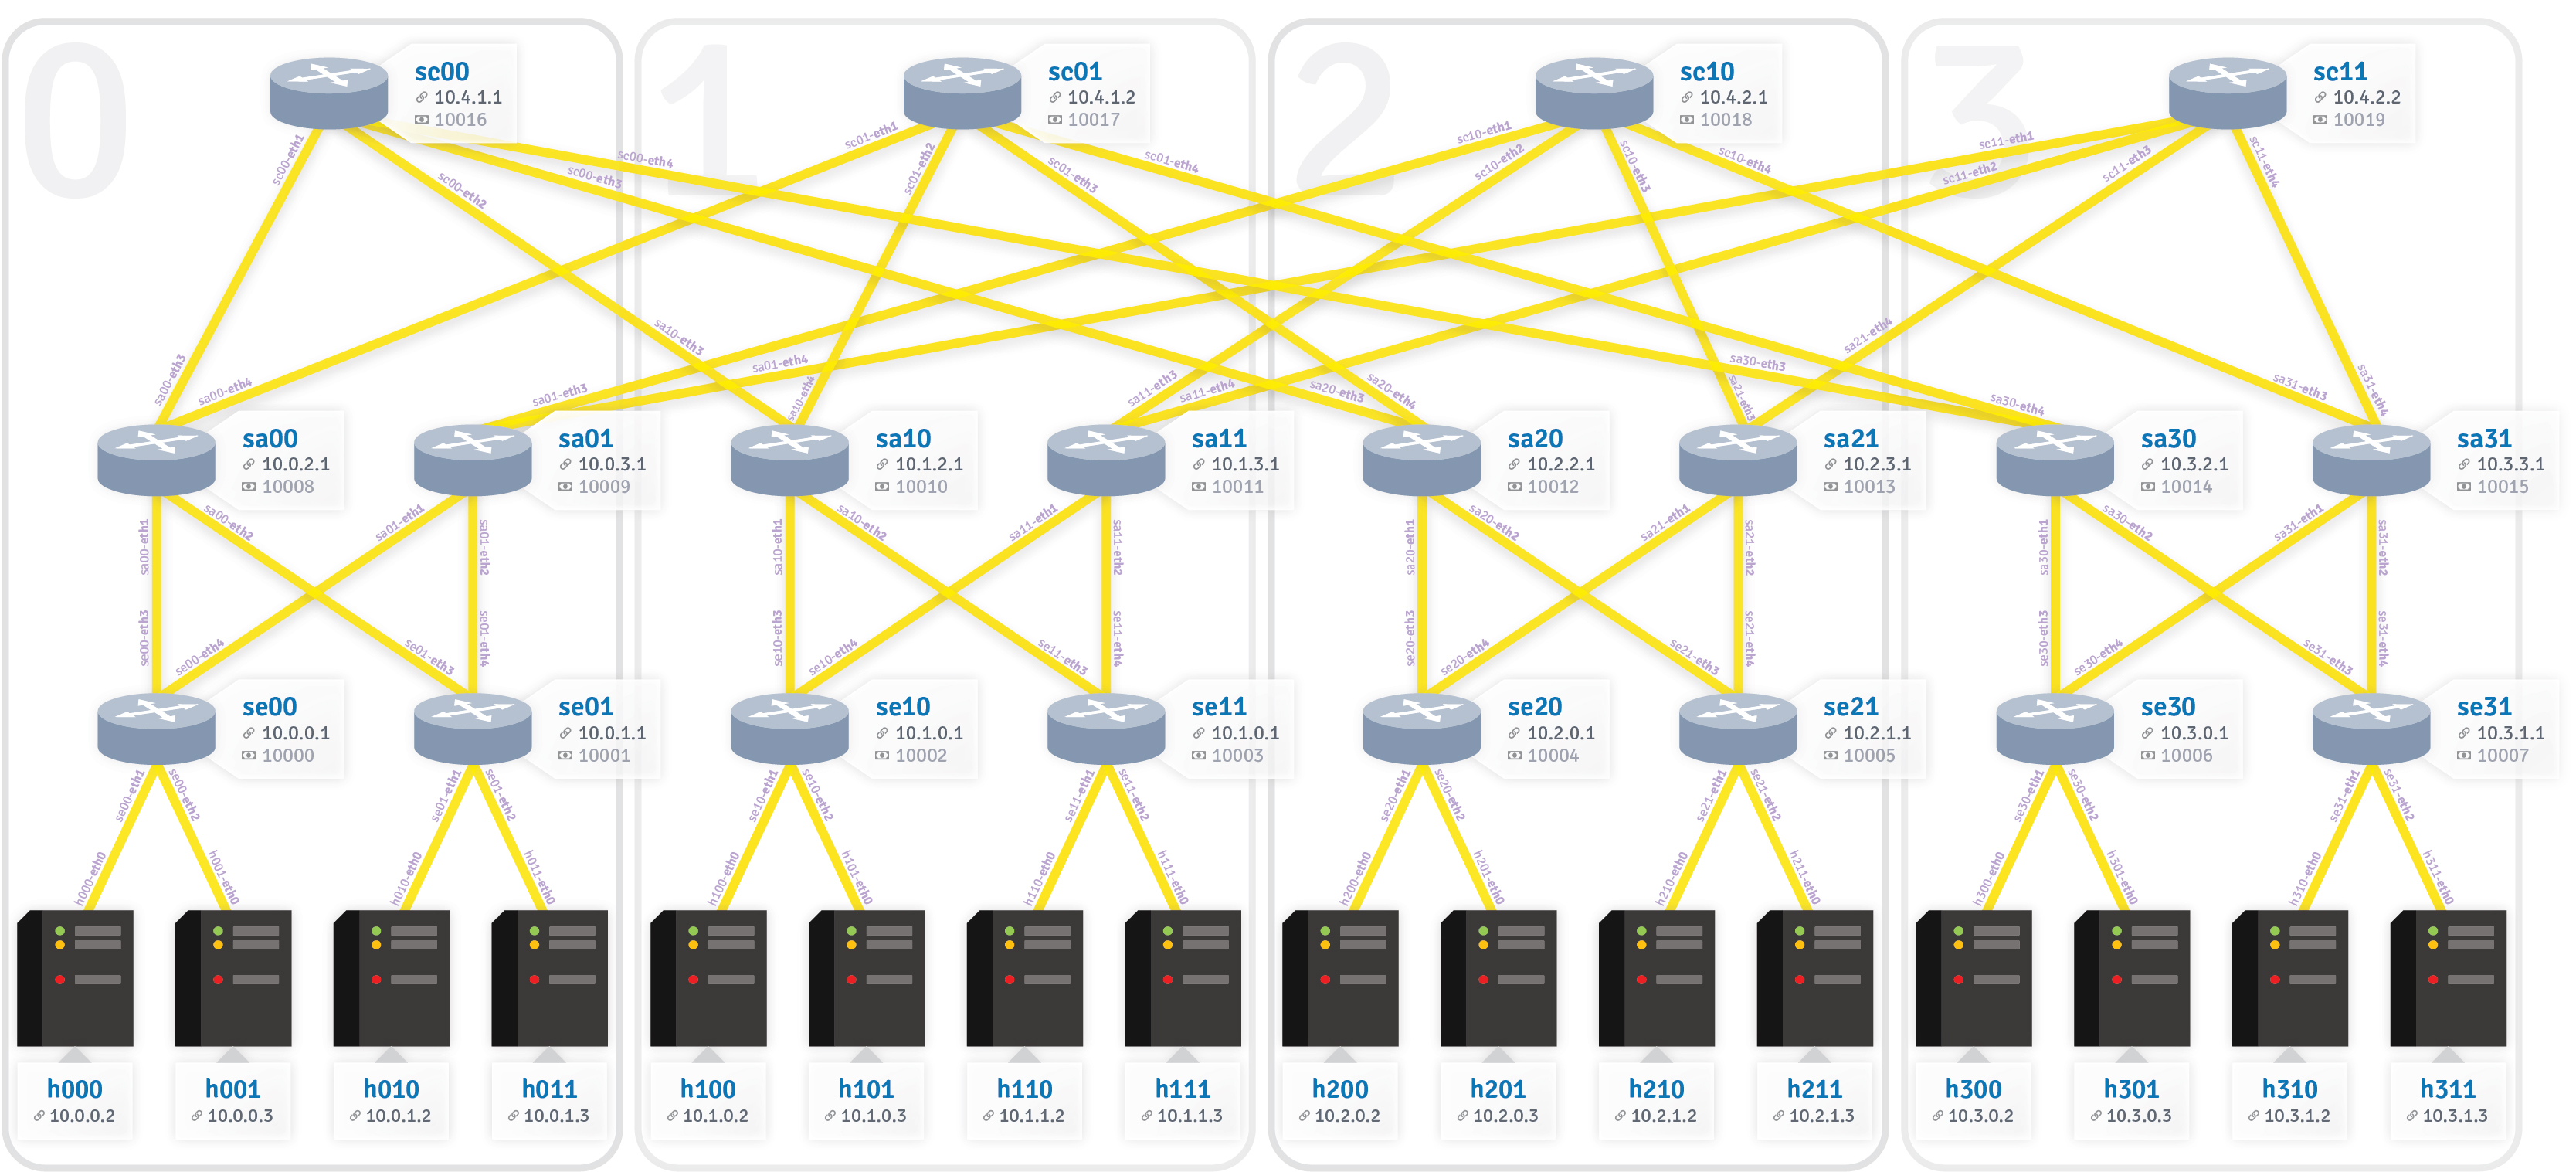
\includegraphics[scale=0.5]{experimenttopo}}
\par\end{centering}
\caption[Fat tree (\code{k = 4}) topology in Mininet.]{Fat tree (\protect\code{k = 4}) topology in Mininet, including naming
and addressing conventions. \label{fig:k-4-topology}}
\end{figure}

The following are the definitions and conventions followed in generating
the topology. 

\subsubsection{Standard Topology Structure}

For a given scaling parameter $K$, the topology is composed of $K$
pods. Each pod is composed of $\frac{K}{2}$ aggregate routers and$\frac{K}{2}$
edge routers, with each aggregate router connected to all edge routers,
and vice versa. Each edge router is connected to $\frac{K}{2}$ hosts,
for a total of $(\frac{K}{2})^{2}$ hosts per pod. There are a total
of $(\frac{K}{2})^{2}$ core routers, each connected to one aggregate
router per pod. 

\subsubsection{Indexes and Names}

The following numbering and naming conventions are used.
\begin{itemize}
\item The pods are numbered for $0$ to $K-1$.
\item Edge routers are named \code{se\textless{}pod\textgreater{}\textless{}i\textgreater{}},
where \code{\textless{}pod\textgreater{}} is the pod id, and \code{\textless{}i\textgreater{}}
is the edge id within the pod, ranging from $0$ to $\frac{K}{2}-1$.
\item Aggregate routers are named \code{sa\textless{}pod\textgreater{}\textless{}i\textgreater{}},
where \code{\textless{}pod\textgreater{}} is the pod id, and \code{\textless{}i\textgreater{}}
is the aggregate id within the pod, ranging from $0$ to $\frac{K}{2}-1$.
\item Core routers are named \code{sc\textless{}i\textgreater{}\textless{}j\textgreater{}},
where \code{\textless{}i\textgreater{}} and \code{\textless{}j\textgreater{}}
ranges from $0$ to $\frac{K}{2}-1$. \code{\textless{}j\textgreater{}}
is an identifier for all cores of the same \code{\textless{}i\textgreater{}},
and \code{\textless{}i\textgreater{}} determines which aggregate
core it connects to for each pod. The significance of \code{\textless{}i\textgreater{}}
and \code{\textless{}j\textgreater{}} are explained in the Links
subsection.
\item Hosts are named \code{h\textless{}pod\textgreater{}\textless{}i\textgreater{}\textless{}j\textgreater{}},
where \code{\textless{}pod\textgreater{}} is the pod id, \code{\textless{}i\textgreater{}}
is the edge id of the edge router it is connected to, and \code{\textless{}j\textgreater{}}
is the host id for all hosts connected to the i'th edge router.
\end{itemize}

\subsubsection{IP Addresses}

From the node names, we can map it directly to unique IP addresses
\cite{al2008scalable}.
\begin{itemize}
\item For hosts with names \code{h\textless{}pod\textgreater{}\textless{}i\textgreater{}\textless{}j\textgreater{}},
the IP address is \code{10.\textless{}pod\textgreater{}.\textless{}i\textgreater{}.\textless{}j+2\textgreater{}}.
\item For edge routers with names \code{se\textless{}pod\textgreater{}\textless{}i\textgreater{}},
the IP address is \code{10.\textless{}pod\textgreater{}.\textless{}i\textgreater{}.1}.
\item For aggregate routers with names \code{sa\textless{}pod\textgreater{}\textless{}i\textgreater{}},
the IP address is \code{10.\textless{}pod\textgreater{}.\textless{}i+(K/2)\textgreater{}.1}.
\item For core routers with names \code{sc\textless{}i\textgreater{}\textless{}j\textgreater{}},
the IP address is \code{10.\textless{}K\textgreater{}.\textless{}i+1\textgreater{}.\textless{}j+1\textgreater{}}.
\end{itemize}

\subsubsection{Links}

The following describes more precisely the connections between nodes\cite{al2008scalable}.
\begin{itemize}
\item An edge router \code{se\textless{}POD\textgreater{}\textless{}I\textgreater{}}
is connected to hosts \code{h\textless{}POD\textgreater{}\textless{}I\textgreater{}\textless{}j\textgreater{}}
for all $0\leq j\leq\frac{K}{2}-1$.
\item All aggregate routers are connected to edge routers in the same pod,
and vice versa. More precisely, an aggregate router \code{sa\textless{}POD\textgreater{}\textless{}I\textgreater{}}
is connected to edge routers \code{se\textless{}POD\textgreater{}\textless{}j\textgreater{}}
for all $0\leq j\leq\frac{K}{2}-1$.
\item A core router \code{sc\textless{}I\textgreater{}\textless{}J\textgreater{}}
is connected to aggregate routers \code{sa\textless{}pod\textgreater{}\textless{}I\textgreater{}}
for $0\leq pod\leq K-1$.
\end{itemize}

\subsubsection{Port Assignment}

Each link connected to a router is assigned a port for that router.
For the following descriptions, the ports are numbered from $0$ to
$K-1$ (though in reality, it is usually numbered from $1$ to $K$).
The following describes the assignment for the p'th port for each
type of router.
\begin{itemize}
\item For an edge router \code{se\textless{}POD\textgreater{}\textless{}I\textgreater{}},
the first $\frac{K}{2}$ ports is assigned to host \code{h\textless{}POD\textgreater{}\textless{}I\textgreater{}\textless{}p\textgreater{}},
and the last $\frac{K}{2}$ ports is assigned to aggregate router
\code{sa\textless{}POD\textgreater{}\textless{}p-(K/2)\textgreater{}}.
\item For an aggregate router \code{sa\textless{}POD\textgreater{}\textless{}I\textgreater{}},
the first $\frac{K}{2}$ ports is assigned to edge router \code{se\textless{}POD\textgreater{}\textless{}p\textgreater{}},
and the last $\frac{K}{2}$ ports is assigned to core router \code{sc\textless{}I\textgreater{}\textless{}p-(K/2)\textgreater{}}.
\item For a core router \code{sc\textless{}I\textgreater{}\textless{}J\textgreater{}},
the ports are assigned to aggregate router \code{sa\textless{}p\textgreater{}\textless{}I\textgreater{}}.
\end{itemize}
The interfaces are similarly assigned, but from \code{eth1} to \code{eth\textless{}K\textgreater{}}
instead of $0$ to $K-1$.

\subsubsection{Thrift Port}

Thrift ports are assigned for each router, and can be used to communicate
and debug with the router. The following describes how the thrift
ports are assigned.
\begin{itemize}
\item The first thrift port is $10000$, and is assigned to \code{se00}.
Succeeding ports are increasing in increments of $1$.
\item The first $K*\frac{K}{2}$ thrift ports are assigned to edge routers
\code{se00, ..., se0\textless{}(K/2)-1\textgreater{}, se10, ..., se\textless{}K-1\textgreater{}\textless{}(K/2)-1\textgreater{}}.
\item The next $K*\frac{K}{2}$ thrift ports are assigned to aggregate routers
\code{sa00, ..., sa0\textless{}(K/2)-1\textgreater{}, sa10, ..., sa\textless{}K-1\textgreater{}\textless{}(K/2)-1\textgreater{}}.
\item The next (and last) $(\frac{K}{2})^{2}$ thrift ports are assigned
to core routers \code{sc00, ..., sc0\textless{}(K/2)-1\textgreater{}, sc10, ..., sc\textless{}(K/2)-1\textgreater{}\textless{}(K/2)-1\textgreater{}}.
\end{itemize}

\subsection{Switch Behavior}

The P4 \code{behavioral-model} repository \cite{p4lang2018behavioral-model}
was forked to get its target executables (e.g., \code{simple\_router})
and modified the source to extend their functionalities (See Appendix
\ref{code-primitives}). Each behavior is defined by tables and actions
coded in C++, and compiled to a JSON using the \code{p4c-bm} tool
\cite{p4lang2018p4c-bm}. The JSON is fed to the target executable,
and the tables are filled with entries during initialization.

\subsubsection{Downstream Packets}

For the following discussions, packets that are forwarded towards
the core (host to edge, edge to aggregate, or aggregate to core) are
considered to be upstream, and otherwise downstream. Since downstream
packets in the fat tree topology have a unique path towards their
destination, each router has only a single correct port to forward
to per destination in the downstream path. Thus, for any switch behavior,
the packet's destination IP Address is matched with a longest prefix
match to check if the packet is headed downstream, and if so forward
it to the appropriate port. All bits are matched for edge routers,
the first 24 bits for aggregate routers, and the first 16 bits for
core routers.

For any router forwarding upstream, each of the $\frac{K}{2}$ upstream
ports to choose from is a valid path. Thus, different switch behaviors
may differ in how packets are forwarded upstream. For this experiment,
three switch behaviors have been implemented - \code{Static}, \code{ECMP},
and \code{PS} (for packet spraying), with \code{Static} serving
as the control. The packet forwarding scheme for each behavior is
discussed in detail in the next subsections.

\subsubsection{Static}

For Static behavior, every destination is assigned to a random port
with equal probability during initialization, and will not change
during runtime (thus the name \code{Static}). Thus, all upstream
paths are matched in the same table as downstream packets, but using
all 32 bits. The P4 code for \code{Static} behavior can be found
in Appendix \ref{code-simple-router}, and the \code{Static} table
entry generation script can be found in Appendix \ref{code-tablegen-simple}.

\subsubsection{ECMP}

For \code{ECMP} behavior, the flow metadata is hashed to determine
the forwarding port. The flow metadata consists of the \code{source IP Address},
\code{source port}, \code{destination IP address}, \code{destination port},
and \code{protocol number}. The hash used is the CRC16 hash function,
and outputs a 3-bit integer.

A 2-parameter matching is done on the table, the first parameter being
the \code{destination IP Address}, and the second parameter being
the output of the hash function. The first parameter is matched using
a longest prefix match, and the second parameter is matched exactly.
For more details, see the P4 code for \code{ECMP} behavior in Appendix
\ref{code-ecmp-router}.

For each downstream port, 8 entries are inserted into the table, one
for each 3-bit integer for the second parameter. Another 8 entries
are inserted for upstream packets, one for each 3-bit integer for
the second parameter, and with \code{0.0.0.0/0} as the first parameter
(match anything). With this setup, downstream ports are matched with
the appropriate entry regardless of the hash value, and those that
aren't matched downstream are matched according to the hash value.
Each 3-bit integer is then assigned to an upstream port in a random
but fair manner i.e. all upstream ports have the same number of hash
values assigned to it, but randomly shuffled. Since we can have at
most 8 hash values, $K$ is limited to at most 16, though this can
be increased when necessary. For more details, see the \code{ECMP}
table entry generation script in Appendix \ref{code-tablegen-ecmp}.

\subsubsection{PS}

For \code{PS} behavior, the chosen upstream forwarding port is chosen
uniformly at random, also known as Random Packet Spraying. According
to the P4 Specifications Document \cite{p4lang2018p4-spec}, uniform
random assignment on a field is a primitive operation, however it
was found that the \code{simple\_router} target in the P4 \code{behavioral-model}
repository \cite{p4lang2018behavioral-model} did not support said
operation. Thus, the source code was modified to extend support, and
the target was recompiled. The modifications can be seen in Appendix
\ref{code-primitives}.

The \code{destination IP Address} is matched with a longest prefix
match to forward downstream packets, similar to Static behavior. In
addition, upstream packets are matched with the entry \code{0.0.0.0/0}
(match all) and corresponds to a special action that assigns a uniformly
random upstream port as the forwarding port. The P4 code for \code{PS}
behavior can be found in Appendix \ref{code-ps-router}, and the PS
table entry generation script can be found in Appendix \ref{code-tablegen-ps}.

\section{Test Design}

To review, the goals of the tests are to measure the network performance
given varying configurations as previously discussed. In particular,
the study will test mainly throughput and flow completion time, with
goodput and mean network utilization as extra data points.

For the purposes of this section, a topology with $K=4$ will be considered.
This means that there are 16 hosts, 16 switches in the edge and aggregate
layers, and 4 switches in the core (see Figure \ref{fig:k-4-topology}).

With this in mind, this allows for 4 unique paths between two hosts. 

\begin{equation}
Given\ k=4,\ paths_{max}=(\frac{K}{2})^{2}=(\frac{4}{2})^{2}=4=n\label{eq:max-paths-1}
\end{equation}
Considering that each host uses only one interface to communicate
to the entire network, preference was given to using \code{ndiffports}
(with $n=4$ ) as MPTCP's path manager in this experiment. This can
be done through the \code{sysctl} feature. The transport protocol
can be changed through \code{net.mptcp.mptcp\_enabled}. Furthermore,
we can control the MPTCP path manager using \code{net.mptcp.mptcp\_path\_manager}.
In this case, we set the path manager of MPTCP-enabled hosts to \code{ndiffports}.

\subsection{Network Traffic Conditions}

Tests were done in two simulated network conditions. The first condition
assumed a network without any activity, allowing for two hosts to
communicate using all of the available resources of the network (hereinafter
referred to as a \emph{silent network}). The second condition assumed
some form of simulated traffic, comparable to the performance in a
live network (hereinafter referred to as a \emph{noisy network}). 

These were done to observe the changes in the design metrics in different
network conditions. Note that the simulation of traffic was an approximation
and may not be representative of the actual datacenter network traffic. 

In the \emph{silent network}, host pairs took turns at sending data
to each other, without any other activity in the network. Pairs were
chosen by random, ensuring that all hosts became a server or client
at some point. The clients requested a payload of certain size from
the server, one after another. This request was then repeated a certain
number of times. The designations were fixed for each iteration of
the test. This was done through a network bandwidth measurement tool
named \emph{iperf}.

\begin{figure}
\begin{centering}
\noindent\resizebox{\textwidth}{!}{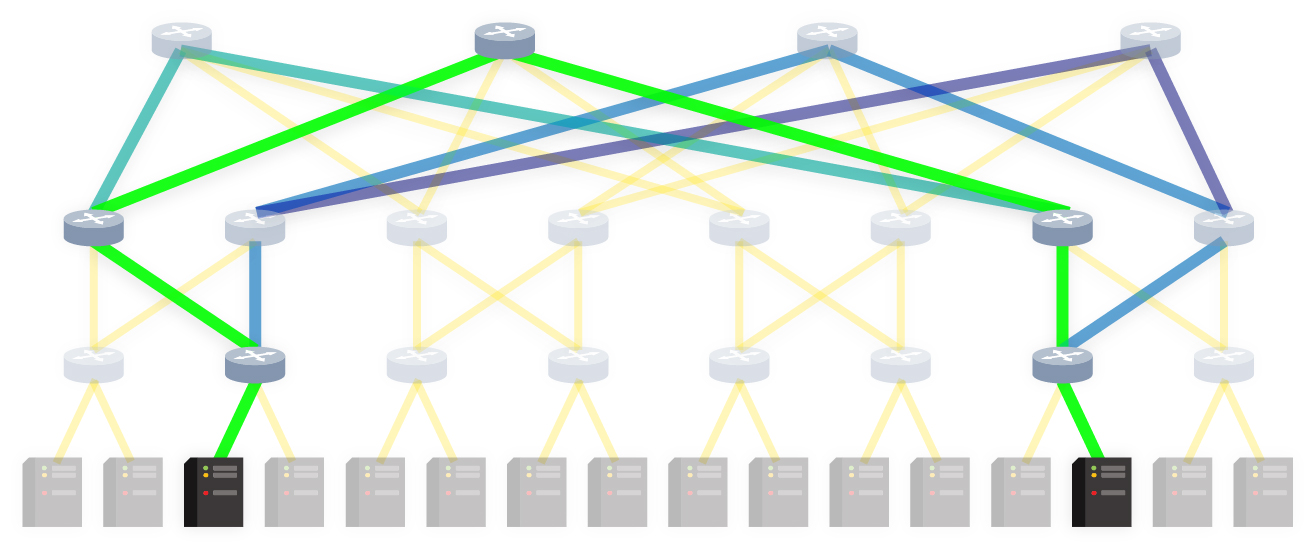
\includegraphics{onetoone}}
\par\end{centering}
\caption[Two hosts communicating in a \emph{silent network} setup]{Two hosts communicating in a \protect\emph{silent network} setup.
Note that there are no other network activity, and that there are
four paths between the two hosts (indicated by the green ang bluish
lines). \label{fig:one-to-one-topo}}
\end{figure}

In the \emph{noisy network}, two hosts requested data from multiple
hosts at the same time, polluting the network with activity. The network
was split between two groups with one client each, and the rest acting
as servers. Considering again a fat tree topology with $K=4$, one
client was chosen at random at the start of the test and seven were
chosen to be file servers. Like the \emph{silent network}, designations
were fixed for each iteration of the test. This was done through an
\emph{HTTP} server in Python, and a tool to transfer data called
\emph{curl}. 

\begin{figure}
\begin{centering}
\noindent\resizebox{\textwidth}{!}{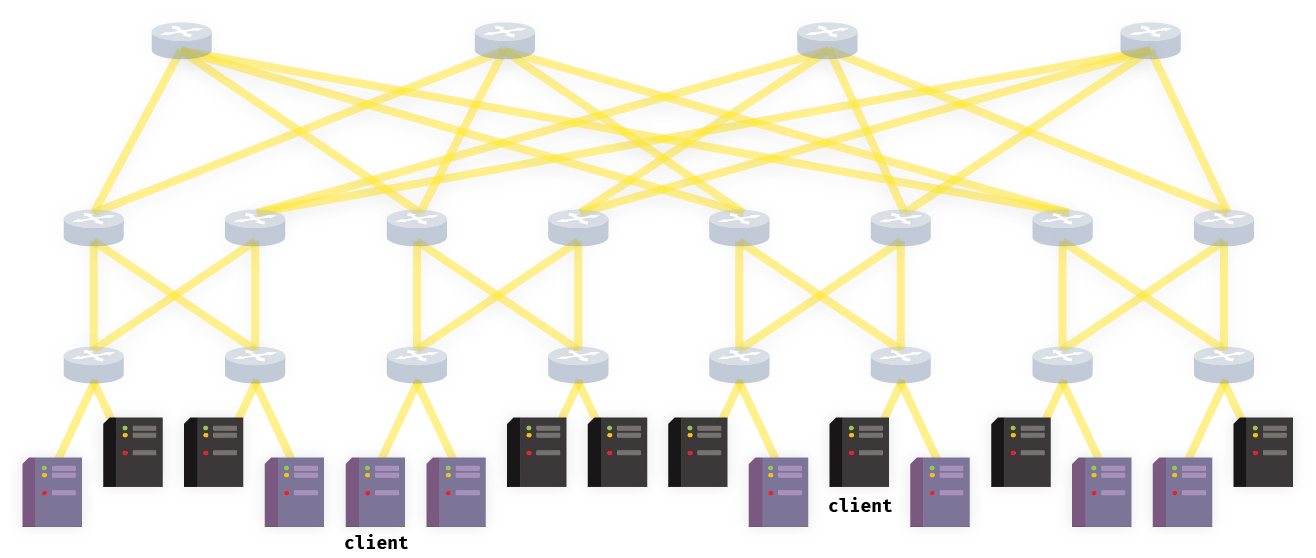
\includegraphics{onetomany}}
\par\end{centering}
\caption[Two host groups in a \emph{noisy network} setup.]{Two host groups in a \protect\emph{noisy network} setup, colored
in black and purple. Note that one host in each group is designated
as the client, to communicate with the rest of the group. \label{fig:one-to-many-topo}}
\end{figure}

In both network conditions, multiple server-client pairs were used
to obtain a thorough assessment of the different links in the network.
Analysis was done through inspection of the packet capture output
of Mininet. Each test is also repeated to obtain a sufficient number
of data points.

\subsection{Test Parameters}

The testbed can have varying permutations of network and host configurations.
To aid in this, the test can be run using different testing parameters
namely, host reorder resiliency, switch behavior, transport protocol,
and payload sizes.

Datacenters cater to requests of varying sizes. To have an approximation
of these requests and how they affect the performance of the changes
to the network stack, we included the option to test with different
payload sizes. Three flow types are to be used and tested for these
experiments: \code{query}, \code{short}, and \code{long} flows
\cite{alizadeh2010data}. 

Note that for the silent network, a query flow is defined with a flow
size of 128KB as the tool used did not allow for the payload size
to go below 128KB. 

\begin{table}
\begin{centering}
\begin{tabular}{|c|c|r|r|}
\hline 
Flow & Examples & Silent Network & Noisy Network\tabularnewline
\hline 
\hline 
query & Quick, bursty connections & 128 kiB & 10 kiB\tabularnewline
\hline 
short & Web page requests & 500 kiB & 500 kiB\tabularnewline
\hline 
long & Streaming, VoIP, file hosting and transfer & 25 MiB & 25 MiB\tabularnewline
\hline 
\end{tabular}
\par\end{centering}
\centering{}\caption[Flow definitions, and their corresponding experimental sizes]{Flow definitions, examples, and their corresponding sizes on both
simulated network traffic conditions.\label{tab:flow-types-defs}}
\end{table}

As a baseline comparison for the improvements of MPTCP, a TCP option
was included in the testing environment. These results served as a
form of control for the performance of MPTCP as a protocol. In addition,
the performance of the changes in the network stack with TCP as its
transport protocol was also measured and analyzed.

\subsection{Performance Metrics}

To review, throughput, goodput, flow completion time, and mean network
utilization between end-hosts were measured to assess the effects
of reorder resiliency in end-hosts and packet spraying in routers.

\subsubsection{Throughput and Goodput}

We define throughput to be the rate of the bytes transferred between
two hosts in the network (i.e., total bytes transferred / flow completion
time). In contrast, goodput is the rate of the actual data (only the
size of the payload) transferred over a period of time (i.e., payload
size in bytes / flow completion time).

A comparison between goodput and throughput can be used to indicate
how much overhead affects the rate of transmission of actual data.
If throughput is higher than goodput, this can be an indication to
the presence of added MPTCP headers or packet retransmissions. This
translates to no perceptible improvement from the perspective of the
hosts.

\subsubsection{Flow Completion Time}

We define flow completion time to be the amount of time that it takes
for a request between two hosts to complete. This includes the first
request packet sent from the client to the server and the last \code{FIN}
packet sent from server to the client.

An increase in flow completion time can be attributed to the overhead
of connection establishment (for MPTCP), packet retransmissions, and/or
\code{ACK} timeouts.

\subsubsection{Mean Network Utilization}

For this paper, we consider mean network utilization to be the ratio
of used links between two hosts. For a fat tree network topology with
$K=4$, there are at most 4 paths that connect two hosts. Ideally,
mean network utilization is maximized if all of paths have the near-equal
(if not equal) minimum amount of bytes transferred in them (i.e.,
all paths have a balanced load with regards to the flow).

\subsection{Statistical Tests}

All in all, the test clusters and independent variables can be summarized
with the following table.

\begin{table}
\begin{centering}
\noindent\resizebox{\textwidth}{!}{%
\begin{tabular}{|c|>{\centering}p{3cm}|>{\centering}p{3cm}|>{\centering}p{3cm}|>{\centering}p{3cm}|>{\centering}p{3cm}|>{\centering}p{3cm}|>{\centering}p{3cm}|>{\centering}p{3cm}|}
\hline 
\multicolumn{3}{|c|}{} & \multicolumn{6}{c|}{Test Clusters}\tabularnewline
\hline 
\multicolumn{3}{|c|}{} & \multicolumn{3}{c|}{Silent Network (1-1)} & \multicolumn{3}{c|}{Noisy Network (1-many)}\tabularnewline
\hline 
\hline 
\multirow{4}{*}{Independent Variables} & \multirow{2}{3cm}{\code{ecmp-mptcp}} & \code{vanilla} & query & short & long & query & short & long\tabularnewline
\cline{3-9} 
 &  & \code{juggler} & query & short & long & query & short & long\tabularnewline
\cline{2-9} 
 & \multirow{2}{3cm}{\code{ps-mptcp}} & \code{vanilla} & query & short & long & query & short & long\tabularnewline
\cline{3-9} 
 &  & \code{juggler} & query & short & long & query & short & long\tabularnewline
\hline 
\end{tabular}
\par\end{centering}
\begin{centering}
}
\par\end{centering}
\centering{}\caption{Test clusters and independent variables used in this experiment.\label{tab:test-sets}}
\end{table}

There are two independent variables: the switch behavior combined
with the underlying transport protocol (\code{ecmp-mptcp}, \code{ps-mptcp}),
as well as the inclusion/non-inclusion of Juggler (\code{juggler},
\code{vanilla} respectively). There are six test clusters, grouped
by network traffic conditions (\emph{silent network}, \emph{noisy network}),
permuted with the three payload sizes (\code{query}, \code{short},
\code{long}). 

There are four dependent variables pertaining to the performance metrics
discussed previously: throughput, goodput, flow completion time, and
mean network utilization.

Each test cluster was subjected to a two-way MANOVA to verify the
significance of the differences, and ranked via comparison of means.
In addition, a comparison of percent differences of goodput and throughput
was executed to inspect the effects of hotspots in the network.

Another experiment was also executed that includes TCP alongside MPTCP
(the addition of \code{static-tcp} and \code{ps-tcp}), to serve
as control. For the majority of the next chapter, we will be discussing
the experiment concerning MPTCP tests only.

\chapter{Results and Analysis}

A proper multivariate analysis of variance (MANOVA) shall be executed
by meeting the following assumptions \cite{noauthor_how_nodate}:
dependent variables should be continuous, independent variables should
consist of two or more categorical groups, there should be independence
between observations, and there should be a sufficient number of data
points. These four assumptions were met by virtue of the experimental
setup. 

Other assumptions for MANOVA, if unmet, reduce the validity of the
results. Some tests show that our data set does not meet some of these
assumptions, which means that the following results should be interpreted
with reservations.

\section{Tests of Between-Subjects Effects and Best Performing Independent
Variables}

We chose a confidence interval of 95\% ($\alpha=0.05$) to determine
the significance of the various test groups. For this chapter, we
will be focusing solely on the tests of between-subjects effects.
Table \ref{tab:manova-p-values} shows the values for each test group.
We then listed the independent variables (Table \ref{tab:manova-best})
with the highest mean for outcomes (Appendix \_\_) that have a significant
result.

\begin{table}
\begin{centering}
\noindent\resizebox{\textwidth}{!}{%
\begin{tabular}{|r|>{\raggedleft}b{3cm}|>{\raggedright}b{3cm}|>{\raggedleft}b{3cm}|>{\raggedleft}b{3cm}|>{\raggedleft}b{3cm}|>{\raggedleft}b{3cm}|}
\hline 
\multicolumn{2}{|r|}{Test Clusters} & \multirow{2}{3cm}{Independent Variables} & \multicolumn{4}{r|}{Dependent Variables}\tabularnewline
\cline{1-2} \cline{4-7} 
Network Traffic Conditions & Flow Type &  & Goodput & Throughput & Flow Completion Time & Mean Network Utilization\tabularnewline
\hline 
\hline 
\multirow{9}{*}{Silent Network (1-1)} & \multirow{3}{3cm}{query} & Switch Behavior + Transport Protocol & 0.640 & 0.888 & 0.310 & \textbf{0.000}\tabularnewline
\cline{3-7} 
 &  & Inclusion of Juggler & \textbf{0.000} & \textbf{0.000} & \textbf{0.000} & 0.675\tabularnewline
\cline{3-7} 
 &  & Combined Interaction & \textbf{0.010} & 0.110 & \textbf{0.009} & 0.230\tabularnewline
\cline{2-7} 
 & \multirow{3}{3cm}{short} & Switch Behavior + Transport Protocol & \textbf{0.007} & 0.571 & 0.057 & \textbf{0.000}\tabularnewline
\cline{3-7} 
 &  & Inclusion of Juggler & \textbf{0.000} & \textbf{0.040} & \textbf{0.000} & 0.133\tabularnewline
\cline{3-7} 
 &  & Combined Interaction & 0.259 & 0.623 & 0.748 & 0.600\tabularnewline
\cline{2-7} 
 & \multirow{3}{3cm}{long} & Switch Behavior + Transport Protocol & \textbf{0.015} & 0.895 & 0.479 & \textbf{0.000}\tabularnewline
\cline{3-7} 
 &  & Inclusion of Juggler & \textbf{0.000} & 0.238 & 0.171 & \textbf{0.001}\tabularnewline
\cline{3-7} 
 &  & Combined Interaction & \textbf{0.000} & \textbf{0.000} & 0.541 & \textbf{0.001}\tabularnewline
\hline 
\multirow{9}{*}{Noisy Network (1-many)} & \multirow{3}{3cm}{query} & Switch Behavior + Transport Protocol & \textbf{0.023} & \textbf{0.008} & 0.127 & \textbf{0.000}\tabularnewline
\cline{3-7} 
 &  & Inclusion of Juggler & \textbf{0.019} & 0.139 & 0.821 & 0.805\tabularnewline
\cline{3-7} 
 &  & Combined Interaction & 0.061 & 0.249 & 0.063 & 0.843\tabularnewline
\cline{2-7} 
 & \multirow{3}{3cm}{short} & Switch Behavior + Transport Protocol & \textbf{0.000} & \textbf{0.000} & \textbf{0.000} & \textbf{0.000}\tabularnewline
\cline{3-7} 
 &  & Inclusion of Juggler & \textbf{0.001} & \textbf{0.000} & \textbf{0.000} & 0.126\tabularnewline
\cline{3-7} 
 &  & Combined Interaction & \textbf{0.005} & \textbf{0.000} & \textbf{0.000} & 0.150\tabularnewline
\cline{2-7} 
 & \multirow{3}{3cm}{long} & Switch Behavior + Transport Protocol & 0.113 & \textbf{0.000} & \textbf{0.008} & \textbf{0.000}\tabularnewline
\cline{3-7} 
 &  & Inclusion of Juggler & 0.374 & \textbf{0.014} & 0.716 & 0.137\tabularnewline
\cline{3-7} 
 &  & Combined Interaction & 0.545 & 0.309 & 0.589 & 0.232\tabularnewline
\hline 
\end{tabular}
\par\end{centering}
\begin{centering}
}
\par\end{centering}
\centering{}\caption[Significance values of each test group in the two-way MANOVA.]{Significance values of each test group in the two-way MANOVA. Significant
tests are marked in bold.\label{tab:manova-p-values}}
\end{table}

\begin{table}
\begin{centering}
\noindent\resizebox{\textwidth}{!}{%
\begin{tabular}{|c|>{\centering}p{3cm}|>{\raggedright}p{3cm}|>{\raggedleft}p{3cm}|>{\raggedleft}p{3cm}|>{\raggedleft}p{3cm}|>{\raggedleft}p{3cm}|}
\hline 
\multicolumn{2}{|c|}{Test Clusters} & \multirow{2}{3cm}{Independent Variables} & \multicolumn{4}{c|}{Dependent Variables}\tabularnewline
\cline{1-2} \cline{4-7} 
Network Traffic Conditions & Flow Type &  & Goodput & Throughput & Flow Completion Time & Mean Network Utilization\tabularnewline
\hline 
\hline 
\multirow{9}{*}{Silent Network (1-1)} & \multirow{3}{3cm}{query} & Switch Behavior + Transport Protocol &  &  &  & ps-mptcp\tabularnewline
\cline{3-7} 
 &  & Inclusion of Juggler & vanilla & vanilla & vanilla & \tabularnewline
\cline{3-7} 
 &  & Combined Interaction & ps-mptcp-vanilla &  & ps-mptcp-vanilla & \tabularnewline
\cline{2-7} 
 & \multirow{3}{3cm}{short} & Switch Behavior + Transport Protocol & ps-mptcp &  &  & ps-mptcp\tabularnewline
\cline{3-7} 
 &  & Inclusion of Juggler & vanilla & juggler & vanilla & \tabularnewline
\cline{3-7} 
 &  & Combined Interaction &  &  &  & \tabularnewline
\cline{2-7} 
 & \multirow{3}{3cm}{long} & Switch Behavior + Transport Protocol & ps-mptcp &  &  & ps-mptcp\tabularnewline
\cline{3-7} 
 &  & Inclusion of Juggler & juggler &  &  & juggler\tabularnewline
\cline{3-7} 
 &  & Combined Interaction & ecmp-mptcp-juggler & ps-mptcp-juggler &  & ps-mptcp\tabularnewline
\hline 
\multirow{9}{*}{Noisy Network (1-many)} & \multirow{3}{3cm}{query} & Switch Behavior + Transport Protocol & ps-mptcp & ps-mptcp &  & ps-mptcp\tabularnewline
\cline{3-7} 
 &  & Inclusion of Juggler & juggler &  &  & \tabularnewline
\cline{3-7} 
 &  & Combined Interaction &  &  &  & \tabularnewline
\cline{2-7} 
 & \multirow{3}{3cm}{short} & Switch Behavior + Transport Protocol & ps-mptcp & ps-mptcp & ps-mptcp & ps-mptcp\tabularnewline
\cline{3-7} 
 &  & Inclusion of Juggler & vanilla & juggler & vanilla & \tabularnewline
\cline{3-7} 
 &  & Combined Interaction & ps-mptcp-vanilla & ps-mptcp-juggler & ps-mptcp-vanilla & \tabularnewline
\cline{2-7} 
 & \multirow{3}{3cm}{long} & Switch Behavior + Transport Protocol &  & ps-mptcp & ps-mptcp & ps-mptcp\tabularnewline
\cline{3-7} 
 &  & Inclusion of Juggler & vanilla &  & vanilla & \tabularnewline
\cline{3-7} 
 &  & Combined Interaction &  &  &  & \tabularnewline
\hline 
\end{tabular}
\par\end{centering}
\begin{centering}
}
\par\end{centering}
\centering{}\caption{Best performing configurations, with non-significant results filtered
out.\label{tab:manova-best}}
\end{table}

For a given link in the network, bandwidth is limited to 20 Mbps.
Tests within a silent network, specifically for throughput, goodput,
and flow completion time are inconclusive as they can maximize the
bandwidth regardless of switch behavior and transport protocol. The
throughput and goodput for a given flow naturally reach the bandwidth
cap in a silent network as there are no other flows competing for
resources.

\section{Gap Between Goodput and Throughput as an Indicator of Network Hotspots}

Network hotspots, defined as switches that have links that are near
to exceed their capacity, result in an increase of dropped packets
and increased packet retransmissions. This results in an increase
in flow completion time, as well as the total amount of bytes transferred.
Therefore, a significant gap between throughput and goodput may be
noticed if network hotspots are in the network. In this experiment,
we took the observed means of goodput and throughput for statically-configured
switches (with hosts running TCP), ECMP-based switches (with hosts
running MPTCP), and PS-based switches (with hosts running TCP and
hosts running MPTCP) and calculated the percentage of traffic in excess
of the actual flow size.

\begin{table}
\begin{centering}
\noindent\resizebox{\textwidth}{!}{%
\begin{tabular}{|c|>{\centering}p{3cm}|>{\raggedleft}p{3cm}|>{\raggedleft}p{3cm}|>{\raggedleft}p{3cm}|>{\raggedleft}p{3cm}|}
\hline 
\multirow{2}{*}{Network Traffic Conditions} & \multirow{2}{3cm}{Flow Type} & \multicolumn{4}{c|}{Switch Behavior and Transport Protocol}\tabularnewline
\cline{3-6} 
 &  & Statically-configured switches (TCP) & Packet Spraying-based switches (TCP) & ECMP-based switches (MPTCP) & Packet Spraying-based switches (MPTCP)\tabularnewline
\hline 
\hline 
\multirow{3}{*}{Silent Network (1-1)} & query & 8.99\% & 10.54\% & 12.96\% & 13.39\%\tabularnewline
\cline{2-6} 
 & short & 9.68\% & 11.41\% & 18.62\% & 17.50\%\tabularnewline
\cline{2-6} 
 & long & 31.69\% & 30.18\% & 35.44\% & 34.47\%\tabularnewline
\hline 
\multirow{3}{*}{Noisy Network (1-many)} & query & 16.29\% & 23.61\% & 31.25\% & 31.65\%\tabularnewline
\cline{2-6} 
 & short & 32.05\% & 43.71\% & 47.69\% & 47.71\%\tabularnewline
\cline{2-6} 
 & long & 51.16\% & 54.37\% & 57.80\% & 58.10\%\tabularnewline
\hline 
\end{tabular}
\par\end{centering}
\begin{centering}
}
\par\end{centering}
\centering{}\caption[Percentage of traffic in excess of \char`\"{}good\char`\"{} traffic]{Percentage of traffic in excess of \char`\"{}good\char`\"{} traffic
(i.e., actual payload size).\label{tab:gap-hotspots}}
\end{table}

If we assume that the percentage of excess traffic is caused by retransmission,
then we can see that statically-configured switches has significantly
less retransmissions over both ECMP-based switches and PS-based switches
for query and short flows. However, during long flows, the difference
between all the switch behaviors seem insignificant. In all cases,
ECMP-based switches and PS-based switches (with hosts running MPTCP)
performed comparably equally, implying that packet spraying did not
mitigate the hotspot problem.

\section{Flow Completion Time Performed Worse with Reorder-Resilient Hosts;
Inconclusive Effects on Throughput}

Since Juggler, the tool to enable reorder-resiliency in the hosts,
was created to increase tolerance between TCP packet arrival times,
it might not perform as well with MPTCP. Based on our results, Juggler
had a negative effect on flow completion time for a silent network
with query and short flows, as well as for a noisy network for short
flows. 

This can also explain the inconclusive results for throughput. Results
are mixed, with Juggler increasing throughput for short flows (on
both silent and noisy networks), but failing to increase throughput
for query flows on a silent network and long flows on a noisy network. 

This leads us to believe that Juggler cannot be simply placed in a
network without negatively affecting its performance.

\section{Packet Spraying Generally Performed Better than ECMP}

As for the switch behavior, packet spraying increased mean network
utilization for all test groups compared to ECMP. In addition, packet
spraying performed better than ECMP for goodput and throughput tests
in a noisy environment. 

This behavior may be preferred as most datacenter networks are high
in network activity.

\section{Effects of Combining Packet Spraying-based Switches with Reorder-Resilient
Hosts}

A combination of packet spraying and reorder resiliency improves throughput
for both silent and noisy networks. However flow completion time increases
(due to the presence of Juggler as seen in the Juggler-only analysis). 

Goodput results turn out to be inconclusive as tests performed better
with PS-based switches, but some preferred the inclusion of Juggler
while others don't. Mean network utilization remains significantly
higher when compared to the rest which can be attributed to the packet
spraying behavior.

\chapter{Conclusion and Recommendations }

Based on preliminary tests, we found that MPTCP increases throughput
significantly compared to TCP, especially with using multiple paths.
However the connection establishment overhead needed to create multiple
subflows penalizes the speed at which flows are created and consequently
completed.

In addition, the paper promised to experimentally prove that ECMP-based
switches causes hotspots in the network. By comparing the throughput
and goodput of ECMP-based switches without reorder resiliency, we
saw that there are was no improvements to the hotspots in the network.
However hotspots in the network may be a consequence of the experiment
setup. This could either be attributed to the amount of traffic in
the noisy network or due to the limited bandwidth at the single interface
of the host for the silent network.

It was also found that packet spraying improves throughput, goodput,
and mean network utilization for a noisy environment. Considering
that most datacenters will, more often than not, operate with a lot
of concurrent flows in the network, packet spraying may be beneficial. 

Packet spraying and reorder resiliency show a significant difference
between groups (except for a noisy network with long and query-length
flows and silent network with short flows). Looking at a noisy network
with short flows, throughput is improved and flow completion time
worsens. 

From this, we can say that packet spraying is better in terms of throughput,
goodput, and mean network utilization. Flow completion time for packet
spraying turned out inconclusive data.

\section{Recommendations and Future Work}

Further analysis may be done on TCP combined with packet spraying
and reorder resilient hosts. According to initial testing, TCP with
reorder resilient hosts and packet spraying showed an increase in
throughput and goodput. This may be promising as there would be no
need to implement a new transport protocol.

Network hotspots may also be studied further by creating a special
testbed specifically built to measure the amount of traffic going
through specific nodes in the network. We hypothesize that packet
spraying may still improve network hotspots caused by ECMP.

Data collected in an datacenter network with real traffic would be
beneficial for the validity of the tests since the simulated traffic
in this experiment is merely an approximation.

\cleardoublepage{}

\bibliographystyle{ieeetr}
\bibliography{Proposal_Part1}
\cleardoublepage{}

\appendix

\chapter{Code Snippets}

These code snippets come from the researchers' git repository available
at \url{https://github.com/MMfSDT/}

\section{Topology Generator - Python Script}

The full repository is available at \url{https://github.com/MMfSDT/mininet-topo-generator}
.

\lstinputlisting[breakatwhitespace=false,breaklines=true,keepspaces=true,columns=flexible,language=Python,numbers=left,caption={mininet-topo-generator/topogen.py, written in Python},label={code-topogen}]{appendix_codes/topogen.py}

\section{Modified P4 - Simple Router Primitives - C++ Script}

The full repository is available at \url{https://github.com/MMfSDT/behavioral-model}.

\lstinputlisting[breakatwhitespace=false,breaklines=true,keepspaces=true,columns=flexible,numbers=left,caption={behavioral-model/targets/simple\_router/primitives.cpp},label={code-primitives}]{appendix_codes/primitives.cpp}

\section{Routers and their Table Generator Scripts - P4 and Python Scripts}

The full repository is available at \url{https://github.com/MMfSDT/behavioral-model}.

\lstinputlisting[breakatwhitespace=false,breaklines=true,keepspaces=true,columns=flexible,numbers=left,caption={mininet-topo-generator/router/simple\_router.p4},label={code-simple-router}]{appendix_codes/simple_router.p4}\pagebreak{}\lstinputlisting[breakatwhitespace=false,breaklines=true,keepspaces=true,columns=flexible,language=Python,numbers=left,caption={mininet-topo-generator/router/tablegen\_simple.py},label={code-tablegen-simple}]{appendix_codes/tablegen_simple.py}\pagebreak{}\lstinputlisting[breakatwhitespace=false,breaklines=true,keepspaces=true,columns=flexible,numbers=left,caption={mininet-topo-generator/router/ecmp\_router.p4},label={code-ecmp-router}]{appendix_codes/ecmp_router.p4}\pagebreak{}\lstinputlisting[breakatwhitespace=false,breaklines=true,keepspaces=true,columns=flexible,numbers=left,language=Python,caption={mininet-topo-generator/router/tablegen\_ecmp.py},label={code-tablegen-ecmp}]{appendix_codes/tablegen_ecmp.py}\pagebreak{}\lstinputlisting[breakatwhitespace=false,breaklines=true,keepspaces=true,columns=flexible,numbers=left,caption={mininet-topo-generator/router/ps\_router.p4},label={code-ps-router}]{appendix_codes/ps_router.p4}\pagebreak{}\lstinputlisting[breakatwhitespace=false,breaklines=true,keepspaces=true,columns=flexible,numbers=left,language=Python,caption={mininet-topo-generator/router/tablegen\_ps.py},label={code-tablegen-ps}]{appendix_codes/tablegen_ps.py}\pagebreak{}

\section{Test Runner Scripts - Bash and Python Scripts}

The full repository is available at \url{https://github.com/MMfSDT/network-tests}.

\lstinputlisting[breakatwhitespace=false,breaklines=true,keepspaces=true,columns=flexible,numbers=left,language=bash,caption={mininet-topo-generator/run.sh},label={code-run-sh}]{appendix_codes/run.sh}

\pagebreak{}

\lstinputlisting[breakatwhitespace=false,breaklines=true,keepspaces=true,columns=flexible,numbers=left,language=Python,caption={network-tests/test.py},label={code-test}]{appendix_codes/test.py}

\pagebreak{}

\lstinputlisting[breakatwhitespace=false,breaklines=true,keepspaces=true,columns=flexible,numbers=left,language=Python,caption={network-tests/postprocess.py},label={code-postprocess}]{appendix_codes/postprocess.py}

\chapter{Experimental Results}

\section{Raw Results}

The test sets were defined at \ref{tab:test-sets}. All results (including
those that included TCP end-hosts), SPSS outputs, and SPSS-ready \code{.csv}
files is available at \url{https://github.com/MMfSDT/thesis-results}.
\end{document}
